\documentclass[a4paper,10pt]{article}
\usepackage{graphicx}
\usepackage{verbatim}
\usepackage{subfig}
\usepackage{float}
\usepackage[spanish]{babel}   %ver bien como es
\usepackage[utf8]{inputenc}
\hyphenation{des-com-po-ner-los va-rie-dad in-gre-dien-tes ac-tua-li-za-cio-nes me-dian-te con-si-de-ra-cio-nes nues-tro au-to-ma-ti-za-do pro-pues-tos con-tras-ta-das ra-zo-na-ble}
\begin{document}

\tableofcontents

\newpage


\section*{Introducci\'on}
\addcontentsline{toc}{section}{Introducci\'on}

El objetivo de este trabajo es brindar posibles soluciones para el desarrollo de un software, el mismo ser\'a utilizado en una cadena de pizzer\'ias llamada "Pizza Hack". El análisis del software a desarrollarse fue solicitado por la cadena, que además puntualizó determinados objetivos que de antemano consideran importantes.


En conjunto con las explicaciones en lenguaje natural se incluyen modelos de objetivos y de agentes. Estos modelos permiten plasmar sintéticamente, de manera gráfica, una idea general de las características que identificamos en el conjunto de las posibles soluciones y que a su vez describen el problema. 

Una de las ventajas de los modelos de objetivos es que permiten identificar las relaciones entre los distintos objetivos de alto nivel, como así también descomponerlos en objetivos más concretos. Ésta descomposición permite a su vez delegar la responsabilidad del cumplimiento de un objetivo en una entidad activa, que se denomina agente, permitiendo de esta manera desarrollar soluciones alternativas con diferente grado de intervención del software en sí. Las alternativas que se generen a partir de la exploración de las posibles soluciones también se podrán ver representadas en forma esquemática. 

En los diagramas de contexto se podrán explorar con más detalle las interacciones que se darían en algunas de las variantes de nuestras posibles soluciones y entender mejor el rol que cumple cada agente.

De acuerdo a los objetivos priorizados por la cadena, el sistema debe tener las siguientes características:


El sistema pedido debe ser un sistema distribu\'ido, es decir, debe operar en cada local por separado. Para realizar este an\'alisis para el posterior desarrollo del sofware se debi\'o pensar en que dicha cadena pretende ofrecer a sus clientes un men\'u en com\'un en todos los locales, es decir, mismo plato y mismo precio. Dicho men\'u debe poder ser modificado, por ejemplo si se desea cambiar alg\'un precio y agregar o quitar alguna variedad de pizza.

Por otro lado, el sistema a desarrollar debe poder tener un manejo del nivel de stock, para que se pueda saber cuando se tienen que reponer los ingredientes. Adem\'as, conocer la cantidad de los elementos necesarios para realizar cada variedad que hay al momento, permite saber si un pedido va a poder ser realizado o no, de esta forma se garantiza que no se cancelen pedidos por falta de ingredientes. En el caso de que el cliente quiera pedir una variedad de pizza que no se pueda realizar en el local donde la est\'a pidiendo, se tiene que poder saber si en alg\'un otro local de la cadena hay stock como para realizar dicho pedido y contar con la posibilidad de reservar los ingredientes, al menos hasta que el cliente la retire en el otro local en cuestion. En el caso de que el cliente no pase a retirar el pedido se tiene que poder recuperar los ingredientes reservados. Finalmente, este informe brinda el an\'alisis de dicho software y requerimientos del hardware para el sistema.


\newpage
\section*{Presunciones}
\addcontentsline{toc}{section}{Presunciones}
En esta secci\'on se describen los fen\'omenos del mundo real que se deben asumir para poder tener un punto de arranque al momento
de pensar las posibles soluciones y no tener la necesidad de analizar las infinitas posibilidades del mundo.

\noindent
\textbf{Tiempo de pedido:} Se asume que dos clientes no pueden hacer un pedido de forma simultánea. Esta presunción permite simplificar el cumplimiento del objetivo relacionado a no dejar que se pueda cancelar un pedido a un cliente luego de que fue hecho, dado que establece un claro orden entre ellos. \\
\textbf{Tiempo de pedido a distancia:} Se asume que, ante un pedido a `distancia' (es decir, de un local a otro), un cliente pierde el interés en buscar dicho pedido luego de un \textit{time out} pautado de antemano. Esta presunción nos ayuda a poder cumplir, por un lado, el objetivo relacionado a permitir dicha compra `a distancia' y, por otro, a poder mejorar el manejo de stock al cancelar el pedido luego de pasado el \textit{time out}, y de esta forma recuperar el stock reservado para éste. Esto se logra sin violar los objetivos relacionados al funcionamiento de las ventas (no cancelar pedidos hechos), dado que se interpreta como que el cliente es el que cancela el pedido al no presentarse y no el local.\\
\textbf{No hay actualizaciones simultáneas:} Habiéndose hecho especial énfasis en que la solución informática no debe ser centralizada, en caso de haber actualizaciones simultáneas se debería arbitrar, de manera distribuída, cuál de las actualizaciones es la que corresponde propagar a la totalidad de las sucursales. Siendo ésta una situación que no consideramos muy común, parece razonable suponer que no hay actualizaciones simultáneas de las variedades del menú. De ésta manera dicho arbitraje no es necesario. \\ 
\newpage

\section*{Vistas}
\addcontentsline{toc}{section}{Vistas}

En esta secci\'on se propondran las soluciones discutidas por el grupo, mediante los diferentes modelos vistos en la materia.
Para esta reentrega se comenzar\'a con el modelo de agentes para mostrar las interraciones entre las diferentes partes en algunas combinaciones de soluciones. Luego se presentar\'a el diagrama de objetivos, el mismo se presentar\'a como un diagrama principal que se ir\'a refinando mediante O-refinamientos e Y-refinamientos para mostrar como las soluciones m\'as chicas interact\'uan para generar la soluci\'on m\'as grande.

Si bien en el trabajo original el orden de los modelos se propuso al reves, para esta reentrega se plantean de este modo para mostrar como es el diagrama de contexto el que muestra un alcance general para luego usar el diagrama de objetivos para explicar cada parte.

\subsection*{Modelo de Agentes}
\addcontentsline{toc}{subsection}{Modelo de Agentes}

El modelo de agentes se caracteriza por sus diagramas de contexto, en los cuales se muestran los diferentes agentes que act\'uan en la soluci\'on y,
a la vez, se muestra la interacci\'on que existe entre estos agentes mediante los fen\'omenos que los relacionan. Dicho esto, se desprende que un
diagrama de contexto solo muestra una posible soluci\'on ya que se trata de una visi\'on global del sistema. Es por esto que se presentan diferentes
diagramas de contexto seg\'un la soluci\'on discutida.

\subsubsection*{Primer Diagrama de Contexto}
\addcontentsline{toc}{subsubsection}{Primer Diagrama de Contexto}
El siguiente diagrama de contexto muestra los agentes involucrados en interacciones con una solución que se orienta a la automatización de la 
mayor\'ia de los problemas a resolver.

\begin{figure}[H]
\centering
\subfloat{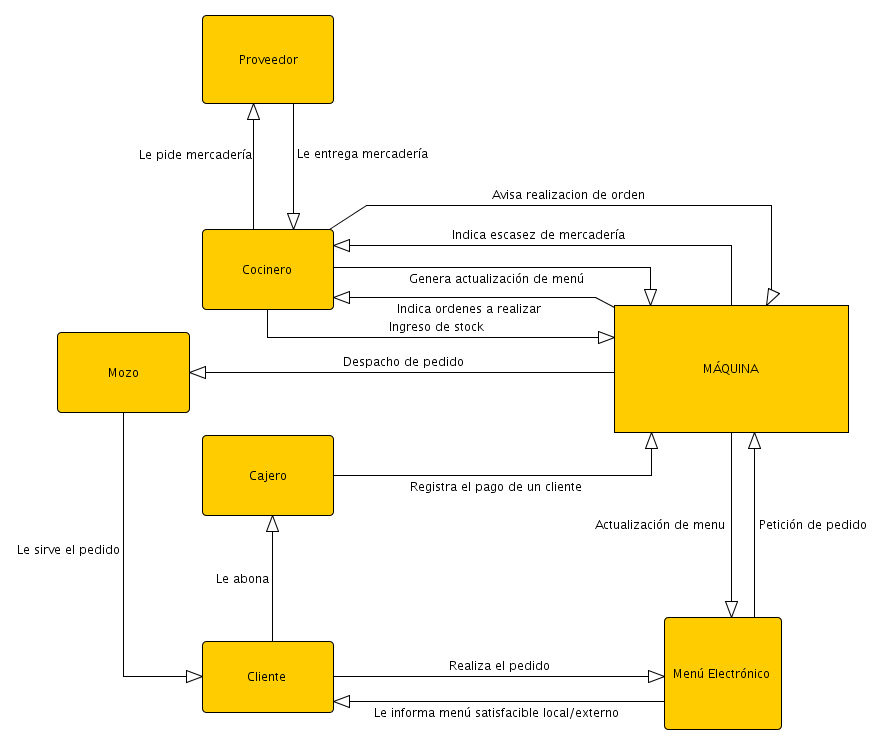
\includegraphics[width=1.0\textwidth]{imagenes/agentes_automatico.png}}
\caption{Diagrama de contexto orientación automatización.}
\end{figure}

\paragraph{Proveedor:}
El proveedor es el encargado de reponer el stock a pedido de nuestro local. Incluye todo el sistema de compra y transporte de productos hasta el local.
\\
\paragraph{Menú Electrónico:}
El menú electrónico consiste en un menú interactivo ofrecido a los usuarios a través de iPADs, los cuales son asignados de a uno por mesa. En éste pueden distinguirse las distintas variedades de productos (no únicamente pizzas, sino también bebidas y postres) y sus correspondientes precios. A su vez, en distintos colores se puede distinguir si el producto está o no disponible (es decir, si hay stock de ingredientes para preparalo) y si, en caso de que no haya, puede o no ser pedido en otro local en que sí haya stock, ofreciéndo al cliente la opción de elegir en qué local puede hacer el pedido.
\\
\paragraph{Cliente:}
El cliente que entra al local. Se refiere tanto a individuos como a grupos.
\\
\paragraph{Personal:}
Se refiere al conjunto de personas que trabajan en el local, éstos son: los mozos, el cajero y los cocineros.
\\

La solución presentada en general prioriza la satisfacción del cliente, ya que al ocuparse el software de manera casi íntegra del manejo de stock, resulta posible descontar inmediatamente la disponibilidad de un determinado ingrediente al registrarse un pedido, incluso antes de iniciarse su preparación. Esto evita que al ocurrir varios pedidos concurrentes se acepten pedidos para los cuáles no se dispone de stock suficiente.

Por otra parte, aún cuando el personal no hubiera registrado la escacez de un ingrediente, el sistema lo informaría logrando la reposición del mismo. Debido a posibles imprecisiones en las cantidades de ingredientes registradas para cada receta es necesario que el personal periódicamente haga un inventario completo de las existencias y actualice las cantidades disponibles mediante una interfaz gráfica que será provista por el software.

Es importante destacar que en este caso estamos considerando la comunicación entre sucursales parte del sistema a desarrollarse. En este sentido este sistema no es completamente tolerante a fallas, ya que en el caso de falla por parte del proveedor de servicio de Internet, el sistema se vería inhabilitado para realizar operaciones entre sucursales. Se podría agregar un modo de funcionamiento manual, pero no garantizaría los beneficios del sistema automatizado y además agregaría costo en concepto de funcionalidades que sólo se utilizarían en caso de falla total del servicio de Internet. 



\subsubsection*{Segundo Diagrama de Contexto}
\addcontentsline{toc}{subsubsection}{Segundo Diagrama de Contexto}

En este caso, el siguiete diagrama de contexto muestra los agentes involucrados en la interaccion con una solucion orientada a mecanismos manuales.

\begin{figure}[H]
\centering
\subfloat{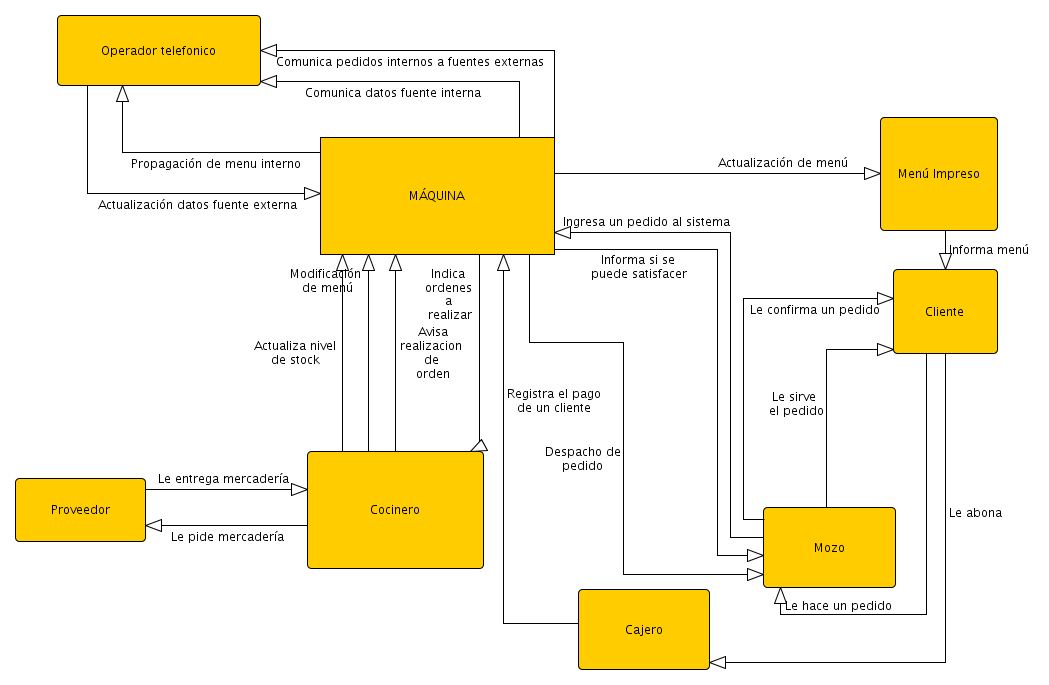
\includegraphics[width=1.0\textwidth]{imagenes/agentes_manual.png}}
\caption{Diagrama de contexto orientación manual.}
\end{figure}

\paragraph{Proveedor:}
El proveedor es el encargado de reponer el stock a pedido de nuestro local. Incluye todo el sistema de compra y transporte de productos hasta el local.
\\
\paragraph{Personal:}
Se refiere a todo el conjunto de personas empleadas en el local. El conjunto tiene una gran interacción con la maquina y con el cliente dado que debe cumplir varias funciones. Actualizar nivel de stock, cuando se hace una nueva compra debe registrarse el cambio. Debe ingresar un pedido al sistema (proveniente de un cliente) para que este evalue si puede o no satisfacerlo. Debe registrar el pago de un cliente. Recibe la confirmación de satisfacción por parte del software, que le indica que puede confirmarle el pedido a un cliente. Tiene también la tarea de pedir al proveedor lo que haga falta corroborando el estado del stock. Debe llevar/recibir/confirmar/servir un pedido.Tiene el deber de actualizar el menu cuando lo crea pertinente.
\\
\paragraph{Cliente:}
Se refiere al cliente que entra al local, tanto a individuos como a grupos.
\\
\paragraph{Menu impreso:}
En esta familia de soluciones, contamos con un menu impreso que debe ser actualizado en todo momento para seguir siendo consistente con la realidad. Cada vez que se quiere actualizar debe ser reeimpreso.
\\
\paragraph{Operador Telef\'onico:}
El operador telef\'onico es el encargado de la comunicaci\'on entre los locales en esta visi\'on manual.
Debe encargarse de actualizar los datos que vienen de afuera y debe informar a las dem\'as pizzerias si un cliente hiz\'o un pedido a distancia en dicha pizzer\'ia, previa consulta de stock. Tambi\'en es el encargado de la propagaci\'on de una actualizaci\'on de men\'u en su propio local. Este alternativa nace como una opci\'on tolerante a fallas como ser\'ia la ca\'ida del servidor de internet en la opci\'on automatizada. 



\subsubsection*{Otras alternativas} 
\addcontentsline{toc}{subsubsection}{Otras alternativas}

En los dos diagramas de contexto anteriores se plasmaron combinaciones espec\'ificas de las soluciones pensadas para los diferentes grupos de
objetivos. Si bien fueron presentados solo dos diagramas de contexto, se podr\'ian realizar muchisimos m\'as mediante la combinaci\'on de las 
soluciones propuestas. Por ejemplo, se podr\'ia idear otro diagrama de contexto, en donde se tenga un sistema de comunicaciones sofisticado resolviendo
todos los problemas de comunicaci\'on, en combinaci\'on con un menu impreso para cada mesa, soluci\'on tan valida como las anteriores.

Por una cuestion de espacio, no se presentan todas las combinaciones posibles, ya que adem\'as no parece aportar nada m\'as a la descripci\'on
de la soluci\'on, dado que los agentes ser\'ian los mismos, pero combinados de otra manera.

\bigskip

\section*{Modelo de objetivos}
\addcontentsline{toc}{subsection}{Modelo de objetivos}

%\centering
%\includegraphics[scale=0.5]{TP1 - Modelo de objetivos - Parte I.png}

\subsection*{Objetivos}
\addcontentsline{toc}{subsubsection}{Objetivos}
\noindent

El siguiente diagrama expresa algunos de los objetivos requeridos por la cadena y que consideramos troncales.

\begin{figure}[H]
\centering
\subfloat{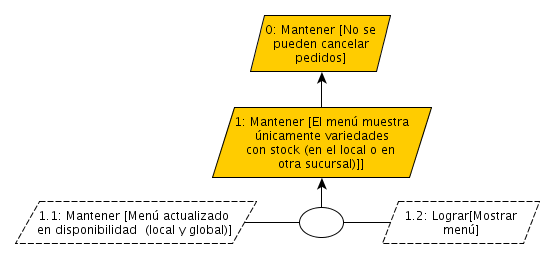
\includegraphics[width=1.0\textwidth]{imagenes/objetivos_principales.png}}
\caption{}
\end{figure}

Los objetivos planteados garantizan que un pedido no será cancelado una vez confirmado. Es decir, un pedido no será cancelado por falta de ingredientes para prepararlo. 

Para lograr esto proponemos que el menú sólo muestre variedades de pizza disponibles, ya sea en la sucursal en la que se está consultando el menú, o eventualmente en otra sucursal, obviamente indicando dicha particularidad. Para esta reentrega tambi\'en se agreg\'o la expectativa de dominio correspondiente a que los clientes solo pueden pedir algo presente en el men\'u.

El objetivo de mantener el menú actualizado en cuanto a disponibilidad plantea a su vez varios objetivos relacionados, por lo que a continuación nos extendemos en su descripción.

\begin{figure}[H]
\centering
\subfloat{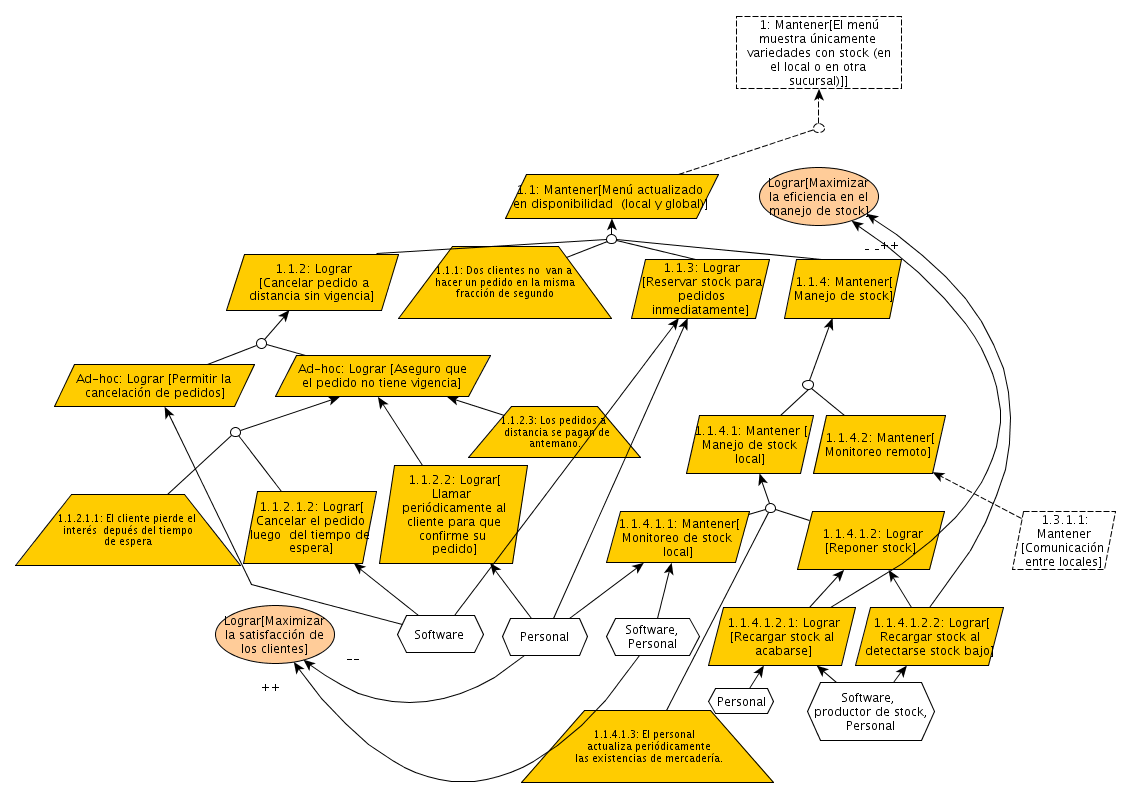
\includegraphics[width=1.0\textwidth]{imagenes/objetivos_menu.png}}
\caption{}
\end{figure}

Como se puede apreciar, surge una gran cantidad de objetivos en algún sentido más simples, algunos de los cuáles consideramos que pueden ser concretados por un agente en particular. En estas asignaciones de objetivos van a surgir las diferentes variantes de la solución propuesta. 

En el anterior diagrama se muestra una dependencia entre el objetivo 1.1 y el 1.1.4. Estrictamente parecería que lo único que es relevante al objetivo 1.1 con respecto al manejo de stock es el monitoreo, tanto local, o restringido a la sucursal en la que se usa el menú, como global, o remoto, del mismo. Por cómo pensamos la solución de software, esta dependencia en realidad existiría, ya que el manejo de stock estaría intimamente ligado a la exactitud y actualidad de los datos obtenidos mediante el monitoreo. Es por eso que mantenemos esa jerarquía.


A continuación nos enfocaremos en el objetivo 1.1.4.1.1. 
\subsubsection*{Mantener [Monitoreo de stock]}
Como vemos, consideramos que existe la opción de asignar la concreción de este objetivo por un lado al Personal, y por otro al Software en conjunto con el Personal. Esta apreciación merece algunas observaciones.
En primer lugar, asignarlo al Personal consistiría en que los cocineros actualicen con cada pedido el stock disponible, descontando manualmente, mediante una interfaz provista por el software, los ingredientes utilizados en cada caso.  


La opción de asignarlo al Software en conjunto con el Personal consiste en que el software asocie cada variedad de pizza a los ingredientes, con sus cantidades correspondientes, necesarios para prepararla. De esta manera, en el instante mismo en que se genera un pedido, el sistema actualizaría las cantidades disponibles de cada ingrediente de manera automática y sin intervención del personal. Sin embargo, por no ser exactas las cantidades registradas en la receta, sería necesario que el Personal haga un inventario completo periódicamente y actualice la disponibilidad de ingredientes con los valores reales.

En este sentido, la expectativa 1.1.4.1.3 tiene varias implicaciones. En el caso de cumplir el objetivo 1.1.4.1.1 con una solución mixta, el Personal debería actualizar las existencias con una periodicidad dada por la eventual inexactitud de las recetas. En el caso de cumplirlo sólo mediante la participación del Personal, sería necesario que la actualización de las existencias fuera casi permanente.

La decisión respecto del objetivo 1.1.4.1.2 está relacionada con las consideraciones mencionadas, ya que, en caso de tenerlo, sería deseable aprovechar las capacidades de monitoreo de stock provistas por el software para alertar al personal de manera que realice un pedido al proveedor si fuera necesario. Las dos políticas de recarga de stock son mencionadas debido a que, si bien la recarga de stock al acabarse es mejor en relación a maximizar la eficiencia en el manejo de stock, ya que se realiza un pedido de mercadería sólo cuando es necesario, es claramente deficiente en relación a la satisfacción del cliente, ya que permite que haya variedades de pizza no disponibles.


La realización de pedidos a distancia, reservando el stock necesario para prepararlo, está relacionada con la precisión del monitoreo de stock. Por lo que ahora nos centraremos en el objetivo 1.1.2:
\subsubsection*{Lograr [Cancelar pedido a distancia sin vigencia]}
Como mencionamos, al realizar un pedido a distancia, los ingredientes para realizar dicho pedido deben ser reservados, garantizando de esa manera que, al llegar el cliente a la sucursal, su pedido todavía puede realizarse. El conflicto surge si un cliente pierde el interés en su pedido y no lo va a retirar.
Este objetivo trae aparejados varios obstáculos, ya que en principio se desearía evitar cancelar un pedido excepto en casos en los que se pudiera asegurar que el cliente perdió el interés en su pedido, pero por otra parte, no es deseable que se mantengan reservados ingredientes que no van a ser utilizados.
Las opciones que a continuación detallamos tienen cada una sus propias ventajas y desventajas, por lo que eventualmente sería necesario que un experto de dominio aporte más información.


Una forma de resolver este conflicto es asumir que los clientes nunca van a retirar su pedido pasado cierto tiempo, debido a que pierden el interés. Siguiendo este razonamiento es seguro volver a disponer de los ingredientes reservados. La limitación de este enfoque es la falta de flexibilidad, ya que un cliente podría retrasarse mucho más de lo común y aún así pasar a buscar su pedido luego de un tiempo considerable.

Una sofisticación de esta idea es requerir información de contacto al realizar un pedido a distancia, un teléfono celular por ejemplo. Y periódicamente llamar al cliente para confirmar que mantiene su interés, dando de baja el pedido en caso contrario. Esta opción, mucho más flexible que la anterior, requiere la participación del Personal y por otra parte requiere que los clientes provean algún tipo de medio de contacto para tener alguna utilidad.

Por último, si los clientes pagaran su pedido en la sucursal en la que se encuentran, aún si el mismo se entregara en otra, sería razonable suponer que lo va a pasar a buscar, por lo que no habría pedidos a distancia que perdieran la vigencia y no sería necesario cancelarlos.

Más adelante retomaremos el objetivo 1.3.1.1, referido a la comunicación entre locales.
El resto de los objetivos tienen nombres lo suficientemente explicativos, por lo que vamos a retomar los objetivos planteados por la cadena.

\begin{figure}[H]
\centering
\subfloat{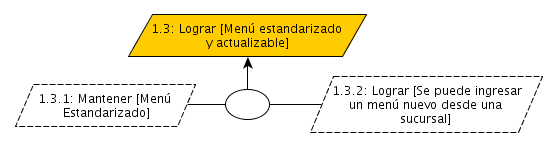
\includegraphics[width=1.0\textwidth]{imagenes/objetivos_menu_estandarizado.png}}
\caption{}
\end{figure}

Entre las pautas se menciona la necesidad de poder actualizar el menú y la restricción de que el menú sea el mismo para todas las sucursales. A continuación nos enfocamos en el objetivos 1.3.1:
\subsubsection*{Mantener [Menú estandarizado]}
para mantener un menú estandarizado simplemente tenemos que aseguranos que sea el mismo en todos los locales, sean cual sean las actualizaciones que se han realizado (de variedades, precios, etc). Para ello únicamente tenemos que asegurar que se mantenga la comunicación entre los locales. \\


\begin{figure}[H]
\centering
\subfloat{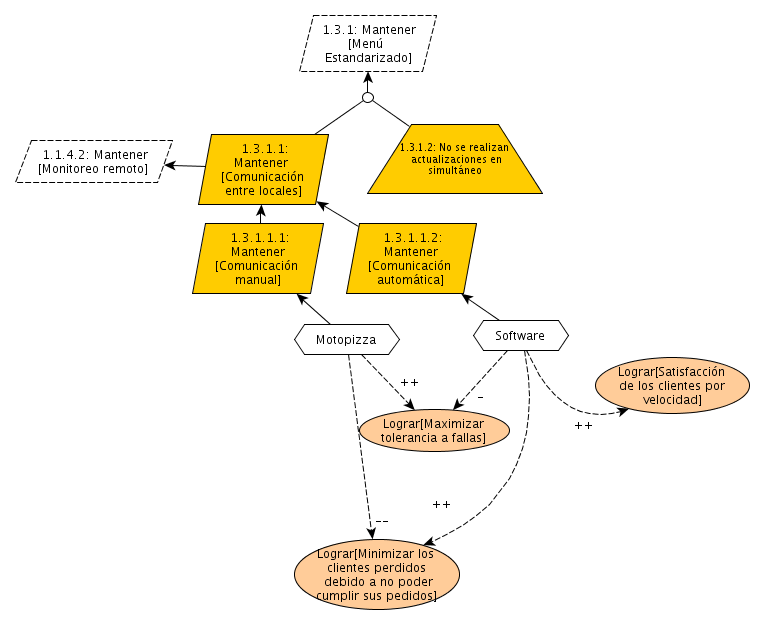
\includegraphics[width=1.0\textwidth]{imagenes/objetivos_menu_estandarizado2.png}}
\caption{}
\end{figure}

La presunción 1.3.1.2 es explicada en mayor detalle en la sección de presunciones.
Las opciones mediante las cuales se puede lograr el objetivo 1.3.1.1 consisten en establecer manualmente la comunicación, entre sucursales o dejarla en manos del software, que operaría a través de internet. 

La opción manual consiste en delegar la tarea de mantener la comunicación a un miembro del Personal, distinguido como operador telef\'onico. 
Como su nombre lo indica, el operador realiza la comunicaci\'on entre los locales mediante el uso del telefono.

Por supuesto, esta solución tiene como defecto principal la velocidad. No se puede, de esta manera, suponer que la información que tenemos de las otras sucursales es absolutamente actualizada, por lo que podrían ocurrir algunos conflictos debidos a este retraso en la transmisión de información. Como ejemplo de esto, ante el pedido de una variedad que se consideraba disponible en uns sucursal remota, este sería autorizado, para luego verificar que la información de la que se disponía era desactualizada. 
Una de las razones que nos hizo considerar la opción manual es su superioridad en términos de tolerancia a fallas. Si esto resulta una característica importante, sería conveniente considerar esta posibilidad.

La solución mediante software ofrece una menor tolerancia a fallas, pero en el caso general garantiza una mayor satisfacción del cliente en cuanto a velocidad, ya que los tiempos de comunicación son mínimos, permitiendo gestionar pedidos a distancia instantaneamente y garantizar que la información compartida es efectivamente la más reciente.

También se da un mejor trato a los clientes, ya que al contar con información actualizada se puede indicar al cliente donde conseguir su variedad preferidad garantizando la no cancelación de su pedido. Esto aporta positivamente a su satisfacción.


%Se debera permitir aceptar pedidos de una sucursal remota y a la vez poder realizar los pedidos que no sean satisfechos pro el local en cuestion a otra sucursal de la cadena que si disponga del stock necesario para cubrir el pedido del cliente.

Para terminar de asegurar la concreción del objetivo 1.3 ahora nos remitimos al objetivo 1.3.2:
\subsubsection*{Lograr [Se puede ingresar un menú nuevo desde una sucursal]}
El ingreso de un nuevo menú plantea un requerimiento con respecto a la funcionalidad del software ya que para tal fin es necesario que se provea de una interfaz que lo permita y algún sistema de autenticación. Este último punto lo consideramos relevante, ya que no sería deseable que por error o mala intención un empleado modificara el menú sin autorización de un superior. A tal efecto se podría utilizar un sistema de administración de usuarios o al menos una contraseña que permitiera acceso a esta funcionalidad restringida.

\begin{figure}[H]
\centering
\subfloat{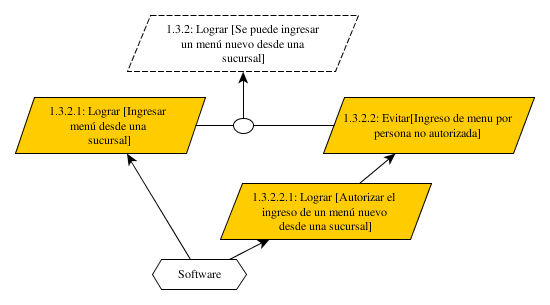
\includegraphics[width=1.0\textwidth]{imagenes/objetivos_menu_ingreso.png}}
\caption{}
\end{figure}

Restaría, para completar el diagrama de objetivos en su totalidad explorar el refinamiento del objetivo 1.2:
\subsubsection*{Lograr [Mostrar menú]}
Para poder adaptarse la información relativa a la disponibilidad, como ser las sucursales en las que se puede pedir una variedad de pizzas agotada localmente, o el repentino cambio de disponibilidad de un plato en particular es necesario considerar la forma en la que vamos a mostrar dicha información.

\begin{figure}[H]
\centering
\subfloat{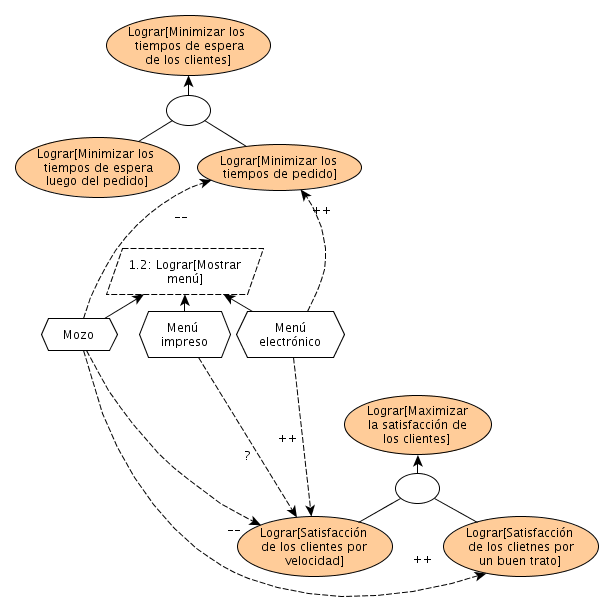
\includegraphics[width=1.0\textwidth]{imagenes/objetivos_menu_mostrar.png}}
\caption{}
\end{figure}

La opción del menú electrónico consiste en un dispositivo similar a una pantalla táctil que permita explorar las variedades, indicando la existencia de disponibilidad o si esto no ocurriese las sucursales que sí pudieran satisfacer el pedido. Esta forma de presentar el menú se integra y complementa con el software. El hecho de que sea una forma tan sofisticada de resolver el asunto tiene aspectos positivos y negativos. Una de las cosas que destacamos es el atractivo que puede generar en la audiencia joven y la mayor satisfacción del cliente a raíz de la disminución de los tiempos de espera. 
Por otra parte, un público de mayor edad podría sentirse intimidado, o preferir la calidez de la interacción con un mozo. En términos de costos esta solución requiere de una inversión inicial más elevada, pero eventualmente reduciría costos operativos a largo plazo debido a la menor cantidad de empleados necesarios para la atención del público. 

Otra opción es delegar en los mozos la responsabilidad de enunciar las variedades disponibles a los potenciales clientes.
Los mozos podrían capacitarse para ofrecer la modalidad de pedido a distancia que posee la cadena. No aprovecharían completamente un sistema de comuninación automatizado ya que sus tiempos de respuesta son incompatibles con los de un sistema informatizado. Por ejemplo, si en una misma sucursal se realizaran varios pedidos de una misma variedad de pizzas en un lapso corto de tiempo un mozo podría estar sugiriendo una variedad para la cual ya no existe disponibilidad. Es relevante destacar que ésta situación no generaría una cancelación en sí, ya que no se permitiría el ingreso del pedido al sistema, resultando en la inmediata notificación del cliente y minimizando su insatisfacción.

Son una solución que aprovecha la tradicional atención personalizada que, aunque no se complemente totalmente con el software, por su muy difundida utilización está probado empíricamente que funciona.

Por último un menú impreso que fuera reemplazado con cada cambio de disponibilidad o de variedades es otra opción. Dependiendo de la frecuencia de la ocurrencia de estos eventos podría ser una solución muy conveniente. 

\bigskip








\newpage
\section*{Escenarios}

Este es un posible escenario de uso, si bien en todo el tp la idea es mostrar variantes para las soluciones, las cuales ser\'ian presentadas 
ante el cliente en cuesti\'on, en este escenario se opt\'o por una soluci\'on para representar como ser\'ia un caso particular.



El dia 29/02/2004 a las 12:47:59 entran simultaneamente al local de pizza Hack (sucursal barrio mitre) Alan Faina, 
Sergio Masa, Tom\'as Anchorena y Laura Oliva en busqueda de una buena sapi. 
Alan se sienta en la mesa nro 1, Tomas en la mesa nro 2, Sergio Masa en la 3 y Laura Oliva en la mesa 4. 

Alan se dispone a pedir su pizza preferida, la de anchoas, toma entonces el men\'u electr\'onico que se encuentra sobre su mesa y
mediante la secuencia de botones Comidas $\rightarrow$ Pizzas $\rightarrow$ Anchoas efectiviza su pedido y queda a la espera del mismo. El pedido se pudo 
realizar porque el monitereo de stock indicaba que la cantidad de anchoas era suficiente para realizar la pizza y, por lo tanto, en el men\'u
esta opci\'on le aparec\'ia a Alan como elegible. Sin embargo, el stock presente solo alcanzaba para una pizza de anchoas, por lo que (el agente
que moniterea el stock) le avisa al personal de la pizzeria que es hora de comprar m\'as anchoas.

Mientras tanto, en la mesa 2, Tomas Anchorena tambi\'en se dispone a pedir su pizza favorita que, al igual que Alan, se trata de la pizza de 
anchoas. Sin embargo, siendo Tomas tan pulcro, no postergo el lavado de sus manos por lo que cuando volvio a su mesa, Alan ya habia realizado
su pedido. Cuando entonces Tomas se dispone a pedir su ansiada pizza de anchoas, comienza a tocar la misma secuencia de botones que Alan. Sin embargo
cuando entra al men\'u de pizzas, se encuentra que el bot\'on correspondiente a la pizza de anchoas esta en gris (es decir, que no es seleccionable).
Tomas, desesperado por su pizza y conociendo el men\'u electr\'onico de la afamada pizzer\'ia, se fija si su pizza se encuentra disponible en otro
local. Pero, al igual que el bot\'on anterior, el bot\'on que indica la opci\'on para pedir pizza en otra sucursal, tampoco se encuentra disponible.

Tom\'as se retir\'a del local, triste por su pizza de anchoas, pero ya haciendosele agua la boca por la fugazzeta rellena de Banchero, su proxim\'o destino.

Por otro lado, Sergio Masa ya se prepara para realizar su pedido en la mesa n\'umero 3. Aunque le cuesta decidirse entre la pizza de morrones
y la de champignones, decide ir con la primera. Cuando Sergio toma su men\'u electr\'onico para pedir la pizza, se da cuenta que el bot\'on 
correspondiente a su elecci\'on no se encuentra en estado seleccionable pero le llama la atenci\'on el bot\'on que se encuentra a un costado. Este
bot\'on predica (Ver disponibilidad en otro local). Sergio toca este bot\'on y en la pantalla aparece un cartel que dice: (Su variedad se encuentra
disponible en el local Belgrano, desea Ordenar?). Sergio muy contento por tener una opci\'on a la falta de morrones en el local, ordena remotamente su pizza
en el local de Belgrano y se dispone a ir a buscarla. 

En ese momento, el pedido de la pizza de morrones llega al local de belgrano y se reserva el pedido, actualizando el stock de la manera adecuada.

Por \'ultimo, Laura Oliva se encuentra en la mesa 4 a punto de pedir una pizza de aceitunas. Laura corre la misma suerte que Sergio dado que el local
de barrio mitre no posee las aceitunas necesarias para realizar la pizza pedida, por lo que Laura ordena remotamente su pizza de aceitunas al local de
Almagro, al cual le llega el pedido remoto.


Luego de 20 minutos, Sergio Masa llega al local de Belgrano y reclama su pizza de morrones, en el local revisan el pedido remoto y cocinan la pizza
pedida. Despues de unos minutos, Sergio se retira feliz con su pizza sobre su mano. 

Luego de otros 40 minutos Laura parece haber cambiado de opini\'on y todav\'ia no aparece por el local de Almagro y
el sistema del local detecta que ya ha pasado una hora desde que Laura Oliva pidio su pizza. Siendo este
tiempo el m\'aximo estipulado para un reserva, el sistema borra la reserva de la pizza de aceitunas y devuelve los potenciales ingredientes
al stock del local, una pizza menos vendida pero por lo menos no se perdieron los ingredientes.



\newpage


\section*{Discusi\'on}
\addcontentsline{toc}{section}{Discusi\'on}

Para la resoluci\'on de este sistema se presentaron distintas alternativas contemplando diversos presupuestos. Las soluciones propuestas son las siguientes:
\begin{itemize}
\item Local manual: Se basa en que la mayor\'ia de la soluciones sean intervenidas por personal y que la interacci\'on con la m\'aquina del mismo sea fuerte.
Siendo los principales objetivos de la maquina, mantener la comunicaci\'on y proveer herramientas para la organizaci\'on del stock por ejemplo.
\item Local automatizado: Se basa en que las soluciones sean mayormente autom\'aticas tanto en el men\'u electr\'onico, como la comunicaci\'on entre locales, como el manejo del stock.
\item Local mixto: Se basa en una mezcla entre el manual y el automatizado. Un caso para esto, ser\'ia por ejemplo tener un men\'u electr\'onico pero que todo lo referente al manejo del stock fuese realizado por personal.
\end{itemize}


Con el men\'u electronico la idea es que a nivel presupuesto sea un gasto grande una vez y despues un minimo costo de mantenimiento. 
Por otro lado, con este tipo de men\'u la idea es que se pueda lograr minimizar los tiempos de pedido(objetivo blando), 
permitiendo eficientemente que cada cliente pueda ver y elegir lo que va a pedir apenas se sientan a la mesa y no tener que esperar a 
que un mozo los pueda atender. De esta forma se puede lograr satisfacci\'on de los clientes por la velocidad (objetivo blando). 


Originalmente se planteo la idea de que hubiese mozos que atendieran a los clientes al ofrecerles un menú cantado.
 Básicamente la idea consistía en que los mozos conocían el menú del día y ofrecían a los clientes las opciones a elegir.
 De esto surgieron varios problemas a considerar, siendo el más grave de ellos el hecho de que, dado que los mozos no tienen datos
 actualizados del stock y dado que cada mozo hace su pedido a la cocina de forma independiente, se pudiesen hacer dos o más pedidos de
 forma simultánea cuando hubiera stock para sólo uno de ellos, de forma tal que se estaría violando el objetivo referente a no poder 
cancelar pedidos. Sin embargo esto no resulta un problema al fin y al cabo, ya que se puede asumir que un pedido se toma como tal, una vez
que el mozo le confirma al cliente que esa pizza esta disponible. Si bien finalmente tener mozos no genera ning\'un problema contra los objetivos
principales, si tienen mucho impacto en los objetivos blandos. El hecho de tener un mozo difiere fuertemente en presentar un men\'u electr\'onico.
El objetivo blando respecto de la satisfacci\'on del cliente podr\'ia verse ayudado o perjudicado por la presencia de un mozo dependiendo el
tipo de cliente. No todas las personas aceptan con naturalidad un dispositivo electr\'onico que resulte de intermediario, prefiriendo un persona. Pero
tambi\'en muchas personas si podr\'ian preferir que no haya mozo, dado que, si se usa correctamente, este dispositivo presentar\'ia una mayor velocidad
a la hora de realizar un pedido.

El punto anteriormente mencionado resulta de gran complejidad de an\'alisis en el mundo real y deber\'ia estar asociado a una consulta con el
experto de dominio para saber que tipo de p\'ublico concurrir\'a a la pizzeria, para de esta manera poder optar por la mejor soluci\'on.

Por otro lado, esta elecci\'on tambi\'en tiene impacto sobre otro objetivo blando que, si bien no aparece en el enunciado, podr\'ia ser perfectamente valido.
El mismo se refiere al costo de mantenimiento. Si bien los dispositivos electr\'onicos podr\'ian resultar en una gran inversi\'on en un primer momento,
abaratar\'ian los costos de funcionamiento luego. En este punto, cabe destacar que esta soluci\'on pertenece al mundo real, en el cual tambi\'en
habr\'ia que analizar si los dispositivos electr\'onicos, una vez funcionando, conservan su integridad conforme pasa el tiempo o no (hurtos, accidentes, da\~{n}o malintencionado).
En el caso de que no conserven su integridad, entonces el costo de mantenimiento seguramente ser\'ia mayor para los dispositivos que para un personal fijo.

\medskip

En cuanto a las dem\'as opciones de soluciones posibles, los impactos sobre los objetivos blandos son, basicamente, an\'alogos a los discutidos
recientemente. Por un lado, podr\'iamos tener el stock controlado por el personal o por la maquina, en este caso la discusi\'on es parecida a la anterior
ya que la versi\'on informatizada ayudar\'ia sobretodo a la velocidad y a la maximizaci\'on de pedidos realizados, mientras que la versi\'on humana
tendr\'ia seguramente un menor costo. En este caso en particular, este aspecto no afectar\'ia a la impresi\'on del cliente, por lo que ser\'ia un
gran factor menos a tener en cuenta.

Por otro lado, la discusi\'on entre sistema de comunicaci\'on informatizada y humana no es tan relevante. En este caso, no cabe ninguna duda que 
solamente un sistema informatizado podr\'ia ayudar a todos los objetivos blandos propuestos, mientras que la soluci\'on humana es nada m\'as una alternativa
tolerante a fallos de la primera.
\medskip

Si bien hay muchos otros aspectos a discutir sobre el impacto de las soluciones sobre los diferentes objetivos, los relevantes ya se realizaron
durante la explicaci\'on del diagrama de objetivos, realizando el an\'alisis pertinente.
 

\newpage
\section*{Conclusiones}
\addcontentsline{toc}{section}{Conclusiones}

En primer lugar, como conclusi\'on principal, se destaca el hecho que si bien el trabajo pr\'actico puede parecer corto en una primera instancia,
lleva varias etapas de discusi\'on entre el grupo, en primer lugar, varias se desarrollaron de manera previa al armado de los modelos, mientras
que muchas otras se generaron durante la marcha.

Para comenzar, lo primero que se hizo, mediante las discusiones mencionadas, fue realizar una lista con los fen\'omenos que abarca este problema
en particular. Luego de realizar esto, el modelo de objetivos pareci\'o la mejor manera de plantear el problema, dado que se puede gu\'iar
fuertemente por las aserciones dadas en el enunciado. Luego, nos abocamos a los diagramas de contexto, donde cada uno representa una interacci\'on
particular entre los agentes.

Para esta reentrega se plantearon los modelos al reves que lo recientemente descripto debido a que se nos marc\'o como importante correcci\'on que la mejor manera de verlo era planteando primero el diagrama de contexto ya que este nos da una visi\'on global de las interraciones y luego, con el diagrama de objetivos, esta visi\'on global se puede ir deslozando en varias partes.


\medskip

Por otro lado, una conclusion importante que destaca el grupo al haber finalizado con el trabajo, es la necesidad que requiere este tipo de
problemas de contrastar con el mundo real. En este caso, nuestra conclusi\'on apunta a que realmente ser\'ia importante poder contar con un 
experto de dominio de por medio para realizar las consultas pertinentes, ya que seguramente el enfoque hubiese cambiado, generando tal vez soluciones
m\'as adecuadas a la realidad de una pizzer\'ia. El hecho de haber obrado nosotros mismos (y los docentes) de experto de dominio, seguramente infieren
sobre las soluciones propuestas.

Otro aspecto que tiene que ver con la falta de un experto de dominio, es algo que nos fuimos dando cuenta durante la realizaci\'on del trabajo pr\'actico.
Al ir refinando sobre los objetivos a realizar, vimos que muchas veces se generaba la duda de si era la maquina la que debia hacerse cargo de
alg\'un problema en particular, o si se deb\'ia asignar a un agente externo. Muchas veces, estos agentes eran humanos, por lo que esos aspectos
quedar\'ian por fuera de una soluci\'on informatizada, teniendo esto sus pros y sus contras. Ser\'ia bueno, poder saber que espera un experto de 
dominio del sistema a desarrollar, si un dominio total del sistema sobre el control de la pizzer\'ia, o bien una herramienta solamente abocada a algunos
aspectos.

\medskip

Por \'ultimo, otra conclusi\'on muy importante a la que se llega mediante este trabajo (la cual esta muy relacionada con la anterior), es que 
si bien las presunciones de dominio parecen razonables, es necesario poder contrastarlas nuevamente con un experto, ya que estas presunciones
tienen un impacto muy fuerte sobre las desiciones tomadas. Nuevamente, estas presunciones fueron contrastadas solamente por los alumnos y los docentes
tratando de que sean lo m\'as razonable posible, sin embargo, lo que nos parece razonable, podr\'ia diferir muchisimo de la realidad en la que 
una pizzer\'ia estar\'ia envuelta.




\end{document}
